%=========================================================================
% Presentation: PyMTL Intro
%=========================================================================

\section[{\it Presentation} PyMTL Intro]{}
\scheduleslide{5}

\begin{frame}{The Design of PyMTL}
\end{frame}

\begin{frame}{Test}
  \centering{%
    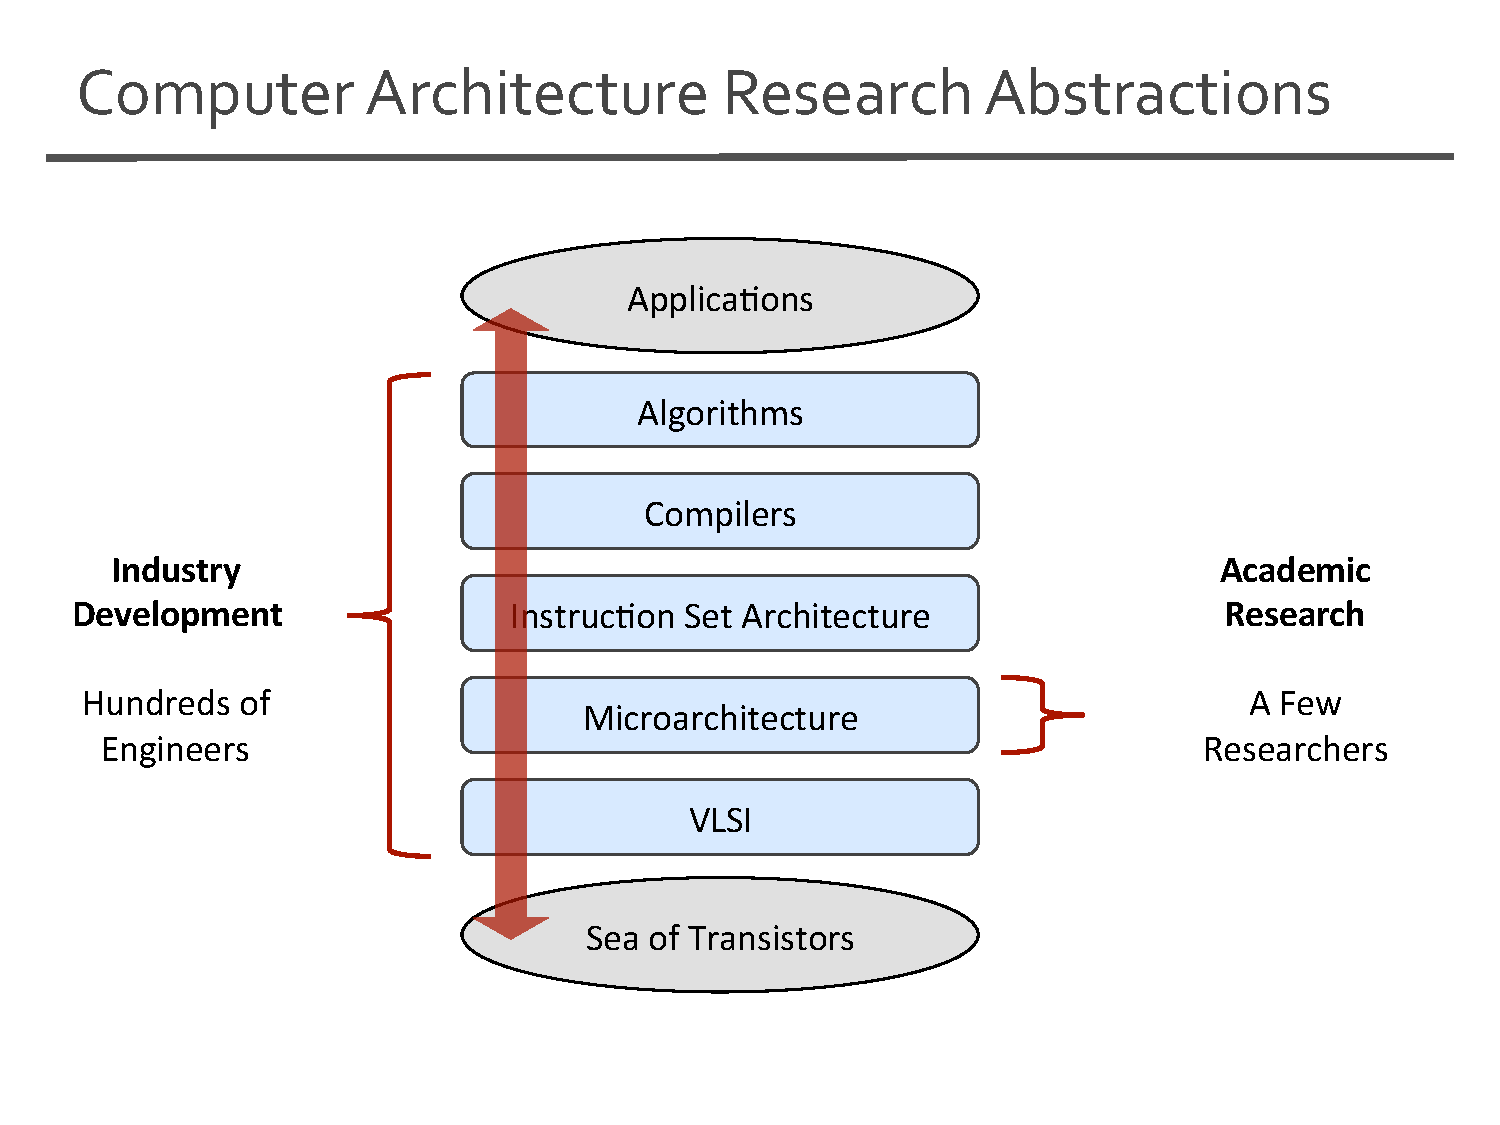
\includegraphics[page=1,trim=0 0 0 1.3in,clip,height=2.85in,keepaspectratio]{../svg/pymtl-intro.pdf}
  }
\end{frame}

\begin{frame}{Computer Architecture Research Abstractions}
 \cbxfigc<1>{../svg/pymtl-abstr0.pdf}
 \cbxfigc<2>{../svg/pymtl-abstr1.pdf}
\end{frame}

\begin{frame}{Computer Architecture Research Methodologies}
 \cbxfigc<1>[.6\tw]{../svg/pymtl-meth0.pdf}
 \cbxfigc<2>[.6\tw]{../svg/pymtl-meth1.pdf}
 \cbxfigc<3>[.6\tw]{../svg/pymtl-meth2.pdf}
\end{frame}

\begin{frame}{Computer Architecture Research Toolflows}
 \cbxfigc<1>{../svg/pymtl-tools0.pdf}
 \cbxfigc<2>{../svg/pymtl-tools1.pdf}
\end{frame}
